\documentclass[UTF8,a4paper,12pt]{ctexart}

\usepackage{geometry}
\usepackage{graphicx}
\usepackage{amsmath}
\usepackage{booktabs}
\usepackage{array}
\usepackage{longtable}
\usepackage{float}
\usepackage{hyperref}
\usepackage{setspace}
\usepackage{indentfirst}
\usepackage{enumitem}
\usepackage{caption}
\usepackage{fancyhdr}

\geometry{left=2.7cm,right=2.7cm,top=2.6cm,bottom=2.6cm}
\hypersetup{colorlinks=true,linkcolor=black,urlcolor=blue}
\setstretch{1.35}
\setlength{\parindent}{2em}
\setlength{\parskip}{0.25em}
\setlength{\headheight}{15pt}
\renewcommand{\arraystretch}{1.25}
\numberwithin{equation}{section}
\captionsetup{font=small,labelfont=bf,labelsep=quad}
\setlist[enumerate]{leftmargin=3em,itemsep=0.2em,topsep=0.2em}
\setlist[itemize]{leftmargin=3em,itemsep=0.2em,topsep=0.2em}
\pagestyle{fancy}
\fancyhf{}
\fancyhead[C]{材料力学专题研究计算说明书}
\fancyfoot[C]{\thepage}
\renewcommand{\headrulewidth}{0.4pt}
\ctexset{
    section = {
        format = \Large\bfseries,
        beforeskip = 1.2ex plus .2ex,
        afterskip = 0.8ex plus .2ex
    },
    subsection = {
        format = \large\bfseries,
        beforeskip = 1.0ex plus .2ex,
        afterskip = 0.5ex plus .2ex
    }
}

\title{材料力学专题研究计算说明书}
\author{}
\date{}

\begin{document}

\begin{titlepage}
    \centering
    \vspace*{2.5cm}
    {\zihao{1}\bfseries 材料力学专题研究\par}
    \vspace{0.8cm}
    {\zihao{2}\bfseries 计算说明书\par}
    \vspace{1.8cm}
    {\zihao{3} 基于 Matlab 的梁弯曲内力、应力与挠度计算程序设计\par}
    \vfill
    \begin{tabular}{rl}
        课程名称： & 材料力学 \\
        作业类型： & 专题研究大作业 \\
        程序文件夹： & \verb|大作业v1| \\
        编写日期： & \today \\
    \end{tabular}
    \vspace*{2.0cm}
\end{titlepage}

\pagenumbering{roman}
\tableofcontents
\clearpage
\pagenumbering{arabic}

\section{选题说明}

本次材料力学专题研究的题目为：基于 Matlab 的梁弯曲内力、应力与挠度计算程序设计。

题目要求如图 \ref{fig:assignment} 所示。

\begin{figure}[H]
    \centering
    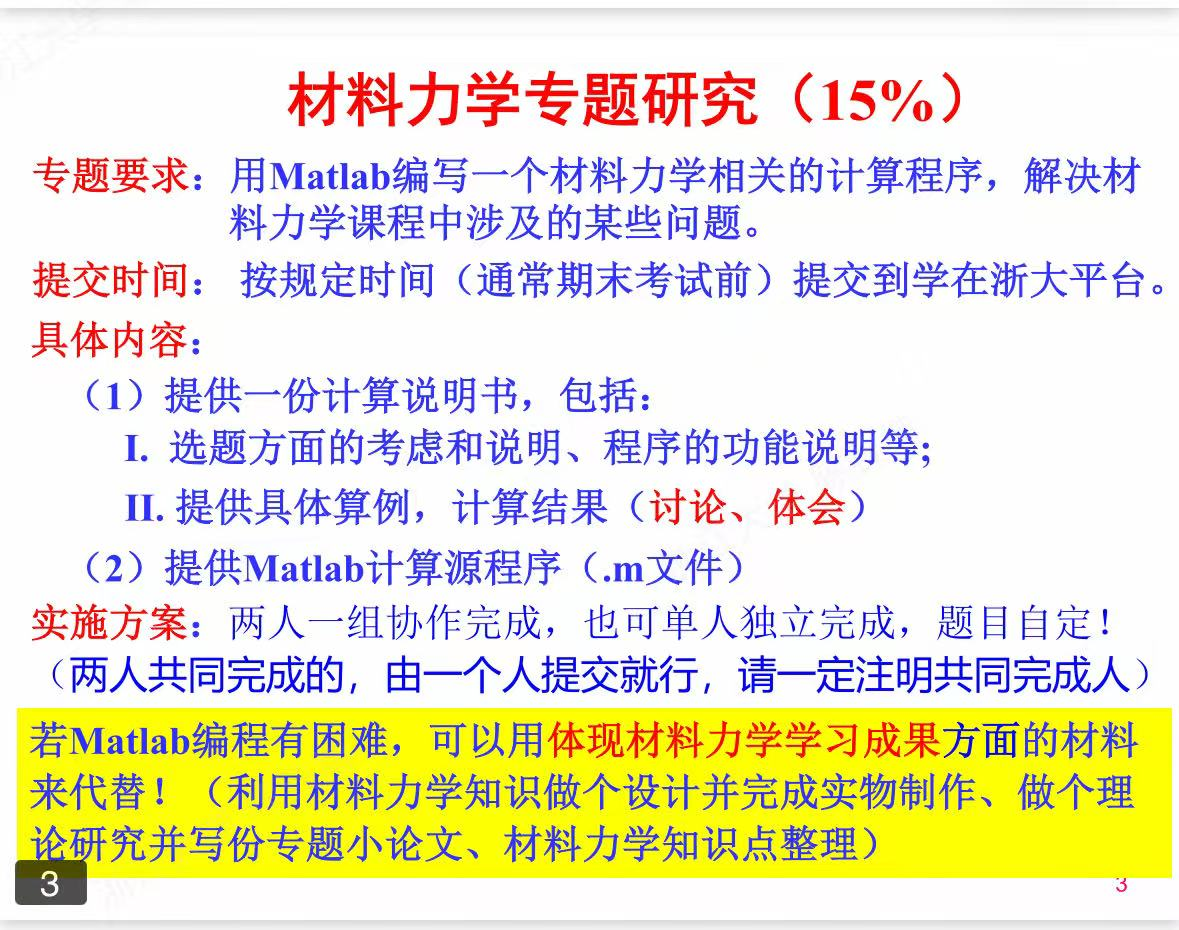
\includegraphics[width=0.85\textwidth]{assignment.jpg}
    \caption{材料力学专题研究要求}
    \label{fig:assignment}
\end{figure}

材料力学课程中，梁的弯曲问题是最常见的结构力学问题之一。对于简支梁、悬臂梁、外伸梁等结构，在受到集中力、集中力偶、均布载荷和线性分布载荷作用时，通常需要计算支座反力、剪力、弯矩、弯曲正应力和挠度。若完全采用手算方法，需要分段建立方程，过程较繁琐，而且容易在载荷分段、符号约定和边界条件处理中出错。

因此，本程序利用 Matlab 编写通用计算工具，将材料力学中的静力平衡、截面法、弯曲正应力公式和 Euler-Bernoulli 梁挠曲线方程结合起来，实现梁弯曲问题的自动计算和绘图。程序源文件存放在 \verb|大作业v1| 文件夹中。

\section{程序功能说明}

程序主要完成以下功能：

\begin{enumerate}
    \item 输入梁的几何参数和材料参数，包括梁长 $L$、弹性模量 $E$、截面惯性矩 $I$、截面边缘到中性轴的最大距离 $y_{\max}$ 和离散计算点数 $n$。
    \item 输入支座类型和支座位置，当前支持简支梁、悬臂梁和外伸梁。
    \item 输入载荷信息，当前支持集中力、集中力偶、均布载荷和线性分布载荷。
    \item 根据整体静力平衡方程计算支座反力。
    \item 沿梁长方向离散，计算每个位置处的剪力 $V(x)$ 和弯矩 $M(x)$。
    \item 根据弯曲正应力公式计算梁截面边缘最大正应力。
    \item 根据梁挠曲线微分方程，采用数值积分方法计算转角和挠度。
    \item 输出关键计算结果，并绘制载荷示意图、剪力图、弯矩图、正应力图和挠度曲线。
\end{enumerate}

\section{程序文件结构}

\begin{longtable}{>{\raggedright\arraybackslash}p{5cm}>{\raggedright\arraybackslash}p{9.2cm}}
\toprule
文件名 & 作用 \\
\midrule
\endhead
\verb|main.m| & 主程序入口，设置一个典型梁算例并输出结果 \\
\verb|interactiveMain.m| & 交互式输入版本，便于用户按提示输入参数 \\
\verb|runExamples.m| & 典型算例验证脚本 \\
\verb|calcReaction.m| & 根据支座和载荷计算支座反力 \\
\verb|calcInternalForce.m| & 计算剪力和弯矩数组 \\
\verb|calcStress.m| & 根据弯矩计算弯曲正应力 \\
\verb|calcDeflection.m| & 由弯矩曲线积分计算转角和挠度 \\
\verb|beamLoadResultants.m| & 将载荷转化为等效集中力、等效作用点和力偶 \\
\verb|beamGetField.m| & 读取结构体字段并提供默认值 \\
\verb|plotBeamResult.m| & 绘制计算结果图像 \\
\bottomrule
\end{longtable}

\section{基本假设与符号约定}

程序采用以下基本假设：

\begin{enumerate}
    \item 梁为等截面直梁，材料均匀、连续、各向同性。
    \item 梁处于线弹性范围内，满足胡克定律。
    \item 梁满足小变形假设。
    \item 横截面变形后仍保持平面，即采用平截面假设。
    \item 不考虑剪切变形对挠度的影响，采用 Euler-Bernoulli 梁理论。
\end{enumerate}

程序符号约定如下：

\begin{enumerate}
    \item 取梁左端为坐标原点，沿梁轴线向右为 $x$ 轴正方向。
    \item 竖直向上的集中力和支座反力取正，竖直向下的载荷取负。
    \item 分布载荷强度 $q$ 也按竖直向上为正，因此常见向下均布载荷取负值。
    \item 剪力和弯矩由截面左侧所有外力累加得到。
\end{enumerate}

\section{理论计算方法}

\subsection{支座反力计算}

对于简支梁和外伸梁，设两个支座位置分别为 $x_A$、$x_B$，反力分别为 $R_A$、$R_B$。将外载荷等效为若干集中力 $F_i$、作用位置 $x_i$ 和集中力偶 $M_j$ 后，整体平衡方程为：

\begin{align}
R_A+R_B+\sum_i F_i &= 0,\\
R_B(x_B-x_A)+\sum_i F_i(x_i-x_A)-\sum_j M_j &= 0.
\end{align}

因此：

\begin{align}
R_B &= -\frac{\sum_i F_i(x_i-x_A)-\sum_j M_j}{x_B-x_A},\\
R_A &= -\sum_i F_i-R_B.
\end{align}

对于左端固定悬臂梁，固定端反力和固定端弯矩由：

\begin{align}
R_A+\sum_i F_i &= 0,\\
M_A+R_A(L-x_A)+\sum_i F_i(L-x_i)+\sum_j M_j &= 0
\end{align}

确定。程序中固定端弯矩 $M_A$ 的取值使自由端内弯矩满足零边界条件。

\subsection{载荷等效处理}

集中力可直接参与平衡方程。均布载荷和线性分布载荷先转化为等效集中力。

对于作用在 $[a,b]$ 区间内的均布载荷 $q$：

\begin{align}
F &= q(b-a),\\
x_F &= \frac{a+b}{2}.
\end{align}

对于线性分布载荷，设起点强度为 $q_1$，终点强度为 $q_2$，作用长度为 $l=b-a$，则：

\begin{equation}
F=\frac{(q_1+q_2)l}{2}.
\end{equation}

合力作用点由载荷图形的一次矩确定。

\subsection{剪力与弯矩计算}

程序沿梁长方向生成离散坐标：

\begin{verbatim}
x = linspace(0, beam.L, beam.n);
\end{verbatim}

然后按照截面左侧外力累加的方式计算剪力和弯矩。集中力 $P$ 作用在 $x_P$ 时，对 $x\ge x_P$ 的截面产生：

\begin{align}
\Delta V &= P,\\
\Delta M &= P(x-x_P).
\end{align}

集中力偶 $M_0$ 作用在 $x_M$ 时，不改变剪力，只使 $x\ge x_M$ 的弯矩发生突变：

\begin{equation}
\Delta M=M_0.
\end{equation}

均布载荷 $q$ 作用在 $[x_1,x_2]$ 区间内时，设某截面左侧已经包含的有效载荷长度为 $l_x$，则其贡献为：

\begin{align}
\Delta V &= ql_x,\\
\Delta M &= ql_x\left(x-x_1-\frac{l_x}{2}\right).
\end{align}

这种处理方式避免了手动分段列式，适用于多个载荷叠加的情况。

\subsection{弯曲正应力计算}

根据材料力学弯曲正应力公式：

\begin{equation}
\sigma=\frac{My}{I}.
\end{equation}

程序关注截面边缘最大正应力，因此取：

\begin{equation}
\sigma_{\max}(x)=\frac{|M(x)|y_{\max}}{I}.
\end{equation}

其中 $y_{\max}$ 为截面边缘到中性轴的最大距离，$I$ 为截面对中性轴的惯性矩。

\subsection{挠度与转角计算}

根据 Euler-Bernoulli 梁理论：

\begin{equation}
w''(x)=\frac{M(x)}{EI}.
\end{equation}

程序先由弯矩数组得到曲率数组，再用梯形积分 \verb|cumtrapz| 积分两次：

\begin{verbatim}
curvature = M ./ (beam.E * beam.I);
theta0 = cumtrapz(x, curvature);
deflection0 = cumtrapz(x, theta0);
\end{verbatim}

数值积分后还需加入两个积分常数。对于简支梁和外伸梁，程序利用两个支座处挠度为零的边界条件：

\begin{equation}
w(x_A)=0,\qquad w(x_B)=0.
\end{equation}

对于左端固定悬臂梁，程序利用固定端转角和挠度均为零的边界条件：

\begin{equation}
\theta(x_A)=0,\qquad w(x_A)=0.
\end{equation}

由此修正转角和挠度曲线，使其满足支座约束。

\section{主程序算例}

\verb|main.m| 中设置的算例如表 \ref{tab:main-case} 所示。

\begin{table}[H]
\centering
\caption{主程序算例参数}
\label{tab:main-case}
\begin{tabular}{ll}
\toprule
参数 & 数值 \\
\midrule
梁长 $L$ & 6.0 m \\
弹性模量 $E$ & 210 GPa \\
截面惯性矩 $I$ & $8.0\times10^{-6}$ m$^4$ \\
边缘距离 $y_{\max}$ & 0.10 m \\
支座类型 & 简支梁 \\
支座位置 & $x_A=0$ m，$x_B=6$ m \\
载荷 & 跨中集中力 $P=-10000$ N，$x=3$ m \\
\bottomrule
\end{tabular}
\end{table}

该问题为标准简支梁跨中集中力问题。由对称性可知：

\begin{equation}
R_A=R_B=5000\ \text{N}.
\end{equation}

最大剪力绝对值为：

\begin{equation}
|V|_{\max}=5000\ \text{N}.
\end{equation}

跨中弯矩最大：

\begin{equation}
|M|_{\max}=\frac{PL}{4}=\frac{10000\times6}{4}=15000\ \text{N}\cdot\text{m}.
\end{equation}

最大弯曲正应力为：

\begin{align}
\sigma_{\max}
&=\frac{|M|_{\max}y_{\max}}{I}\\
&=\frac{15000\times0.10}{8.0\times10^{-6}}\\
&=1.875\times10^8\ \text{Pa}=187.5\ \text{MPa}.
\end{align}

跨中最大挠度理论值为：

\begin{align}
|w|_{\max}
&=\frac{PL^3}{48EI}\\
&=\frac{10000\times6^3}{48\times210\times10^9\times8.0\times10^{-6}}\\
&=2.6786\times10^{-2}\ \text{m}=26.79\ \text{mm}.
\end{align}

程序输出的剪力、弯矩、应力和挠度曲线应与以上理论结果一致。由于程序采用离散点数值积分，最大值位置和挠度值可能存在很小的离散误差。

\section{典型算例验证}

\subsection{算例一：简支梁跨中集中力}

该算例与主程序相同，用于验证简支梁反力、剪力、弯矩和跨中挠度计算。

\begin{table}[H]
\centering
\caption{简支梁跨中集中力算例结果}
\begin{tabular}{ll}
\toprule
项目 & 结果 \\
\midrule
$R_A$ & 5000 N \\
$R_B$ & 5000 N \\
最大剪力绝对值 & 5000 N \\
最大弯矩绝对值 & 15000 N$\cdot$m \\
最大正应力 & 187.5 MPa \\
最大挠度绝对值 & 26.79 mm \\
\bottomrule
\end{tabular}
\end{table}

结果说明：剪力图在跨中集中力处发生突变，弯矩图为两段直线，跨中弯矩最大；挠度曲线关于跨中对称，跨中挠度最大。

\subsection{算例二：悬臂梁自由端集中力}

算例参数如表 \ref{tab:cantilever-param} 所示。

\begin{table}[H]
\centering
\caption{悬臂梁自由端集中力算例参数}
\label{tab:cantilever-param}
\begin{tabular}{ll}
\toprule
参数 & 数值 \\
\midrule
梁长 $L$ & 2.0 m \\
弹性模量 $E$ & 210 GPa \\
截面惯性矩 $I$ & $8.0\times10^{-6}$ m$^4$ \\
边缘距离 $y_{\max}$ & 0.10 m \\
支座类型 & 左端固定悬臂梁 \\
载荷 & 自由端集中力 $P=-2000$ N \\
\bottomrule
\end{tabular}
\end{table}

计算结果如表 \ref{tab:cantilever-result} 所示。

\begin{table}[H]
\centering
\caption{悬臂梁自由端集中力算例结果}
\label{tab:cantilever-result}
\begin{tabular}{ll}
\toprule
项目 & 结果 \\
\midrule
固定端竖向反力 $R_A$ & 2000 N \\
固定端弯矩 $M_A$ & -4000 N$\cdot$m \\
最大剪力绝对值 & 2000 N \\
最大弯矩绝对值 & 4000 N$\cdot$m \\
最大正应力 & 50.0 MPa \\
自由端最大挠度绝对值 & 3.175 mm \\
\bottomrule
\end{tabular}
\end{table}

其中自由端挠度按理论公式计算为：

\begin{align}
|w|_{\max}
&=\frac{PL^3}{3EI}\\
&=\frac{2000\times2^3}{3\times210\times10^9\times8.0\times10^{-6}}\\
&=3.175\times10^{-3}\ \text{m}.
\end{align}

结果说明：悬臂梁最大弯矩和最大应力均出现在固定端，自由端弯矩为零，自由端挠度最大，符合材料力学理论。

\subsection{算例三：简支梁局部均布载荷}

算例参数如表 \ref{tab:udl-param} 所示。

\begin{table}[H]
\centering
\caption{简支梁局部均布载荷算例参数}
\label{tab:udl-param}
\begin{tabular}{ll}
\toprule
参数 & 数值 \\
\midrule
梁长 $L$ & 8.0 m \\
弹性模量 $E$ & 210 GPa \\
截面惯性矩 $I$ & $8.0\times10^{-6}$ m$^4$ \\
边缘距离 $y_{\max}$ & 0.10 m \\
支座类型 & 简支梁 \\
均布载荷 & $q=-3000$ N/m，作用区间 $x=2$ m 到 $x=6$ m \\
\bottomrule
\end{tabular}
\end{table}

均布载荷等效合力为：

\begin{equation}
F=q(6-2)=-12000\ \text{N}.
\end{equation}

由于载荷关于跨中对称，支座反力为：

\begin{equation}
R_A=R_B=6000\ \text{N}.
\end{equation}

跨中剪力为零，跨中弯矩最大：

\begin{align}
M_{\max}
&=6000\times4-\frac{3000(4-2)^2}{2}\\
&=18000\ \text{N}\cdot\text{m}.
\end{align}

最大正应力为：

\begin{align}
\sigma_{\max}
&=\frac{18000\times0.10}{8.0\times10^{-6}}\\
&=2.25\times10^8\ \text{Pa}=225\ \text{MPa}.
\end{align}

按分段弯矩函数积分并利用简支梁边界条件，可得到跨中最大挠度约为：

\begin{equation}
|w|_{\max}=6.7857\times10^{-2}\ \text{m}=67.86\ \text{mm}.
\end{equation}

结果说明：该算例验证了程序对局部均布载荷的处理能力。剪力图在均布载荷区间内呈线性变化，弯矩图在载荷区间内呈二次曲线变化，最大弯矩和最大挠度均位于跨中。

\section{结果讨论}

从上述算例可以看出，程序计算结果与材料力学经典公式一致，说明程序中支座反力、剪力弯矩、应力和挠度计算流程是正确的。

程序的主要优点是：

\begin{enumerate}
    \item 通过结构体统一描述梁、支座和载荷，输入形式较清晰。
    \item 将载荷统一转化为对剪力和弯矩的叠加贡献，减少了手工分段推导。
    \item 同一套计算流程可以处理多种载荷组合。
    \item 结果可视化直观，有助于理解剪力图、弯矩图和挠度曲线之间的关系。
\end{enumerate}

程序也存在一些不足：

\begin{enumerate}
    \item 当前挠度采用数值积分，结果精度受离散点数 $n$ 影响。
    \item 当前悬臂梁版本主要支持左端固定形式，其他固定位置还可继续扩展。
    \item 程序主要考虑静定梁，对连续梁等超静定结构尚未实现。
    \item 当前只计算弯曲正应力，尚未进一步计算剪应力和强度校核安全系数。
\end{enumerate}

\section{心得体会}

通过本次大作业，我将材料力学中梁弯曲问题的理论公式转化为 Matlab 程序实现。编程过程中最关键的是统一符号约定和载荷处理方式。如果符号约定不统一，支座反力、弯矩图和挠度方向很容易出现矛盾。通过将集中力、力偶和分布载荷分别写成对剪力和弯矩的贡献，可以使程序逻辑更加清楚。

另外，挠度计算体现了理论推导和数值方法之间的联系。弯矩函数经过两次积分得到转角和挠度，但积分常数必须由边界条件确定。程序中利用支座处挠度为零或固定端转角、挠度为零来修正积分结果，这与手算挠曲线方程的思路是一致的。

本次作业不仅加深了我对支座反力、剪力图、弯矩图、弯曲正应力和挠度曲线的理解，也提高了使用 Matlab 解决工程计算问题的能力。

\section{结论}

本程序完成了一个材料力学梁弯曲计算工具，能够对常见静定梁在多种载荷作用下的反力、剪力、弯矩、弯曲正应力和挠度进行计算与绘图。通过三个典型算例验证，计算结果与材料力学理论公式一致，满足本次专题研究中“用 Matlab 编写材料力学相关计算程序并提供计算说明书和具体算例”的要求。

\end{document}
